%----------------------------------------------------------------------------------------
%	ANALISI ARCHITETTURALE
%----------------------------------------------------------------------------------------

\section*{Analisi architetturale}
\addcontentsline{toc}{section}{\protect\numberline{}Analisi architetturale}%
\label{sec:analisi_architetturale}

In questo capitolo verranno presentate le decisioni architetturali inerenti la struttura e l'organizzazione del software di simulazione. L'analisi comincia con una visione generale della gerarchia di eventi, per poi suddividersi nelle scelte che riguardano la parte di concorrenza e le scelte che riguardano la parte di distribuzione.

\subsection*{Gli eventi}
\addcontentsline{toc}{subsection}{\protect\numberline{}Gli eventi}%
\label{sec:analisi_eventi}

Gli eventi sono l'elemento costituente di una partita. Essi possono essere generati dalle diverse entita' e possono essere raggruppati in diverse categorie. Inoltre, alcuni di questi eventi sono interessano la sola parte concorrente, mentre altri eventi possono viaggiare dalla parte concorrente a quella distribuita e viceversa.

\begin{figure}
	\centering
	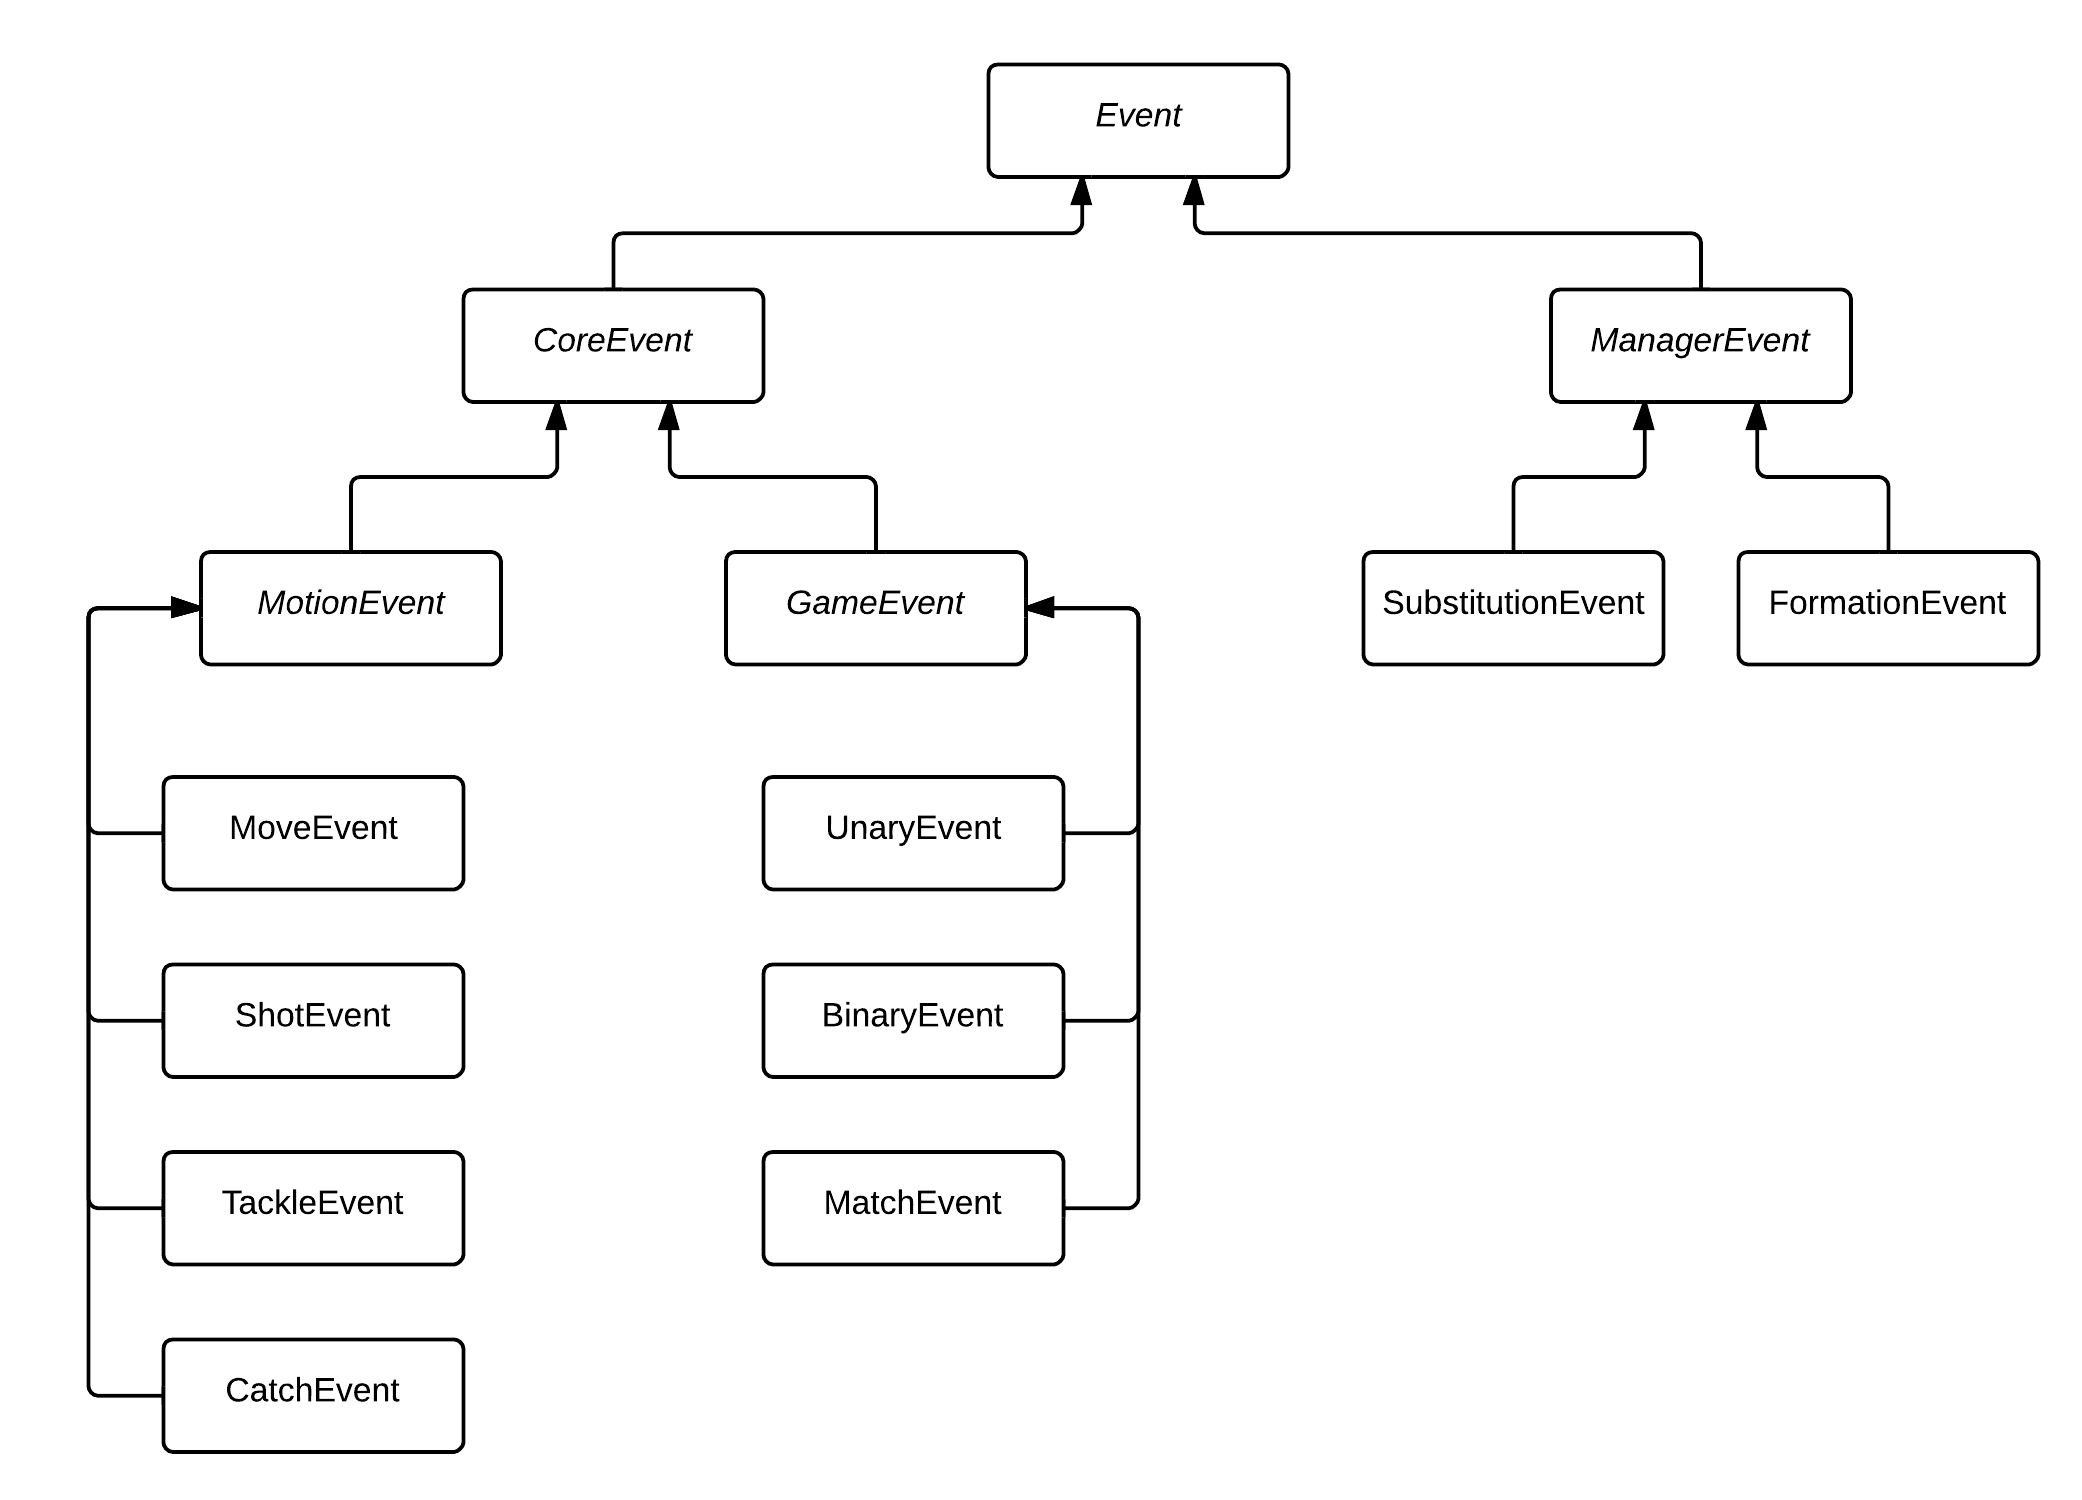
\includegraphics[scale=.5]{images/event_hierarchy.png}
	\caption{La gerarchia degli eventi che costituiscono una partita.}
	\label{fig:event_hierarchy}
\end{figure}

La struttura globale degli eventi e' schematizzata in Figura~\ref{fig:event_hierarchy}. Data la sua complessita' ed estensione, verranno ora trattati singolarmente i diversi tipi di eventi al fine di spiegarne il loro significato e il contesto in cui vengono utilizzati.

\paragraph{Event} \textit{Event} rappresenta l'evento generico ed e' alla base della gerarchia. Da esso si diramano due macro-categorie di eventi: i \textit{CoreEvent} e i \textit{ManagerEvent}. Esso sono rispettivamente gli eventi che vengono generati nella parte concorrente (il cosiddetto ``Core'') e gli eventi che vengono generati nella parte distribuita (fondamentalmente, dagli allenatori). \textit{Event} puo' essere considerata come un'entita' astratta, che non viene concretizzata se non da uno dei suoi derivati.

\paragraph{CoreEvent} Gli eventi di tipo \textit{CoreEvent} sono un insieme di eventi che vengono generati dalla parte concorrente del sistema, ovvero il Core. La loro generazione tuttavia non vincola il loro utilizzo nella sola parte concorrente: essi vengono infatti inviati alla parte distribuita per notificare gli allenatori (e l'interfaccia grafica del campo) sullo svolgersi della partita. Vi sono due tipologie di \textit{CoreEvent}: i \textit{MotionEvent}, che rappresentano le possibili azioni dei giocatori, e i \textit{GameEvent}, che invece rappresentano tutti quelli eventi che influiscono sullo stato di gioco. Anche in questo caso, i \textit{CoreEvent} sono astratti e trovano una concretizzazione nei loro discendenti.

\paragraph{MotionEvent} Tutte le azioni che un giocatore puo' compiere sono definite dai \textit{MotionEvent}. Sono stati definiti quattro tipi di \textit{MotionEvent}, elencati di seguito.

\begin{itemize}
	\item \textit{MoveEvent} - Descrivono i movimenti di un giocatore, dal punto in cui si trova al punto in cui si vuole spostare. Questi eventi vengono altresi' usati per descrivere gli spostamenti della palla.
	\item \textit{ShotEvent} - Rappresentano il tiro/passaggio effettuato da un giocatore, e sono caratterizzati da alcune informazioni quali la posizione del giocatore e la potenza impressa alla palla.
	\item \textit{TackleEvent} - Corrisponde al tentativo di contrasto verso un altro giocatore.
	\item \textit{CatchEvent} - Questo evento descrive il gesto di prendere possesso di una palla, sia essa inerte sul campo (non in possesso) oppure come intercettazione di una palla in movimento.
\end{itemize}

Ciascuno di questi eventi viene sottoposto all'attenzione dell'arbitro, che ne valida la correttezza nel rispetto delle regole del gioco. Inoltre, come gia' anticipato, questi eventi vengono anche inviati alla parte distribuita, cosi' da poter aggiornare la visualizzazione della partita e per permettere agli allenatori di prendere decisioni tattiche.

\paragraph{GameEvent} Gli eventi che regolano lo svolgimento del gioco rientrano nella categoria di \textit{GameEvent}.

\subsection*{Concorrenza}
\addcontentsline{toc}{subsection}{\protect\numberline{}Concorrenza}%
\label{sec:analisi_concorrenza}

Le dinamiche che regolano le interazioni tra le entita’ nello scenario di gioco sono state discusse nel modello, in questa sezione vengono messe in risalto le scelte architetturali relative alla concorrenza, cioe’ come vengono effettivamente gestiti i vari interleaving e gli accorgimenti utilizzati per risolvere le varie criticita’.\\

Per poter meglio comprendere le scelte architetturali che caratterizzano in particolar modo la gestione dello stato da parte del controllore e’ opportuno soffermarsi su alcune considerazioni che vedono protagoniste alcune entita’ in gioco.\\

Si ricorda che le operazioni di lettura non richiedono mutua esclusione, sono quindi richieste potenzialmente eseguibili in modo parallelo. Al contrario in caso di scrittura vi e’ bisogno di mutua esclusione, in alcuni caso si sfrutta la potenza di un particolare tipo di canale per accodare richieste e processarle solamente al verificarsi di determinate situazioni. [non so se ha senso, casomai la scrivo piu’ meglio se dite che ci sta]

\subsubsection*{Palla}
\addcontentsline{toc}{subsubsection}{\protect\numberline{}Palla}%
\label{sec:analisi_concorrenza_palla}

Nel capitolo precedente e’ stata approfondita la tematica della palla e dell’agente di movimento. All’interno dell’architettura e’ stato deciso di tenere le informazioni riguardanti la palla slegate rispetto al controllore, vediamo quindi le motivazioni di questa scelta. Nelle dinamiche viste finora tutte le informazioni di gioco sono detenute nello stato e gestite dal controllore, questo significa che gli accessi sono in mutua esclusione e le richieste di aggiornamento processate in ordine di arrivo, ognuna delle quali deve quindi attendere lo smaltimento delle coda. Questo particolare e’ utile nel caso dei calciatori, e’ uno degli aspetti che riflettono il realismo del gioco, ci sono giocatori piu’ veloci ed altri piu’ lenti, ma questo argomento verra’ ripreso in uno dei paragrafi successivi. Al contrario la palla dev’essere slegata da questa sequenzialita’ che lega i giocatori, ed essere libera di muoversi quando vuole ed alla velocita’ desiderata. Queste considerazioni hanno portato alla decisione di tenere le stato e palla separate, in modo tale da permettere a quest’ultima di muoversi liberamente durante un passaggio o un tiro.\\

Come detto in precedenza, la palla puo’ essere in due stati, inerte o in movimento, quest’ultimo a sua volta si divide in due parti, movimento causato da giocatore e da parte dell’agente di movimento. La struttura della palla e’ stata quindi studiata in modo tale da permettere ad un entita’ alla volta di poterla controllare, quindi o uno dei giocatori o l’agente di movimento.

\subsubsection*{Giocatori}
\addcontentsline{toc}{subsubsection}{\protect\numberline{}Giocatori}%
\label{sec:analisi_concorrenza_giocatori}

Si e’ deciso che i giocatori siano stateless, quindi che non abbiano coscienza del proprio stato di gioco in modo permanente, bensi’ ad ogni turno deve richiedere al controllore informazioni su se stesso oltre che dell’ambiente circostante. La necessita’ di avere un unico luogo di sincronizzazione in cui detenere tutte le informazioni di gioco ha reso inutile, nonche’ ridondante, avere le stesse informazioni anche all’interno di ogni giocatore. Inoltre questa soluzine avrebbe reso ancor piu’ complicato avere uno stato generale della partita sempre aggioranto e consistente.\\

Come detto in precedenza, ogni giocatore e’ caratterizzato da delle statistiche che lo differenziano dagli altri, ed ha come scopo quello di rendere lo svolgimento del gioco piu’ realistico. Tali statistiche comprendono potenza, velocita’, contrasto, difesa, attacco, precisione e bravura in porta. In particolare queste caratteristiche, abbianate allo stato di gioco dello stesso giocatore, rendono possibile effettuare alcune assunzioni che influiscono nello svolgimento del resto del turno. Questo aspetto risultera’ piu’ semplice con un esempio; se un giocatore possiede la palla e tra le proprie statistiche ha un’alta precisione e potenza, esso potra’ effettuare un lancio lungo, in caso contrario potra’ optare un passaggio corto ad un compagno vicino. Viene definita in questo modo un’area di interesse del giocatore, entro la quale esso potra’ agire con l’azione che deve ancora decidere di eseguire. Alla luce di queste considerazioni, un giocatore che chiede al controllore lo stato di gioco della partita non necessita di avere una visione globale dell’intero campo, bensi’ solamente di una sua sotto parte.\\

La parte iniziale di ogni turno del giocatore risulta’ cosi’ suddivisa:\\

\begin{enumerate}
	\item richiesta al controllore del proprio stato di gioco
	\item dove si trova la palla
	\item richiedere al controllore lo stato della propria area di interesse.
\end{enumerate}

La seconda fase consistenza nella parte di intelligenza artificiale, che date le informazioni ottenute decide quale mossa effettuare, questo argomento verra’ trattato nell’apposito capitolo. Una volta decisa la mossa da effettuare, viene creato il relativo evento a cui abbina un certo livello di priorita’, cioe’ quanto e’ importante per il giocatore l’azione appena decisa. Nel paragrafo successivo viene discusso cosa succede da questo momento in poi, cioe’ quando l’azione viene sottoposta al controllore per andare a modificare lo stato.\\

Antecedente al ciclo di turni che caratterizzano la normale esecuzione di un giocatore e’ presente una fase di inizializzazione nella quale il giocatore attende che tutti i giocatori siano attivi, recupera il proprio id ed attende l’inizio della partita.\\

Come nel caso precedente, vi sono altri momenti della partita in cui il giocatore deve essere fermato in attesa di un evento che faccia riprendere il normale svolgimento del gioco, un esempio e’ la pausa tra la fine del primo tempo e l’inizio del secondo. In questi casi viene fatto uso di una risorsa protetta che mette a disposizione dei canali per accodare i giocatori per poi sboccarli all’avvenire di determinate condizioni.

\subsubsection*{Stato, controllor ed arbitro onniscente}
\addcontentsline{toc}{subsubsection}{\protect\numberline{}Stato, controllore ed arbitro onniscente}%
\label{sec:analisi_concorrenza_controller_arbitro}

Lo stato consiste in una serie di dati che descrivono ogni giocatore in campo, quindi un identificativo, il numero di maglia, la posizione attuale e quella di riferimento in campo (cioe’ la posizione dettata dalla formazione). Lo scopo delle azioni da parte dei giocatori e’ quella di andare a modificare la propria posizione all’interno del campo ed effettuare altre operazioni ai fini del gioco.\\

Il controllore e’ di fermare e far partire il gioco, la sua componente di arbitro, nonche’ le interazioni con l’utente, permettono di regolare l’andamento del gioco, ed e’ proprio bloccando la ricezione di richieste scrittura di eventi che si ha l’effetto play / pause della partita.\\

Ogni richiesta viene presa in cosiderazione dalla componente che rappresenta l’arbitro, il quale valuta la correttezza o meno dell’azione. In caso di fallo l’arbitro ferma il gioco dal punto di vista logico e sancisce la squadra per il prossimo possesso palla. A questo punto prima che il gioco possa riprendere l’arbitro attende prima di tutto che le squadre si riposizionino correttamente per garantire le giuste distanze dal punto di battuta, poi il gioco riprende effettivamente al momento di battuta da parte del giocatore designato.\\

Nella sezione che parla degli eventi e’ stata data una panoramica delle operazioni possibili da parte dei giocatori, dal punto di vista del controllore vengono gestite in modo differente: una volta accettata la richiesta, esso determina il tipo di evento e cerca di soddisfare il giocatore permettendogli di andare aggiornare lo stato con l’azione richiesta. Il fatto che il giocatore divida il suo turno in fasi, fa in modo che i presupposti secondi cui ha scelto una determinata mossa al momento non vi siano piu’. Per esempio, un giocatore tenta di prendere la palla che e’ in una certe posizione, ma tra quando se ne e’ accorto e quando tenta effettivamente di prenderne il possesso, la palla si e’ spostata. Questo, come anche in altri casi in cui ha senso applicare questo tipo di comportamento, e’ dettata dal tentativo di creare una simulazione realistica, se un giocatore non e’ abbastanza veloce o si accorge tardi di una certa circostanza e’ giusto che veda la propria azione fallire.\\

Se l’operazione fallisce il controllore si comporta in modo differente in base al tipo di operazione richiesta: operazioni come il passaggio, il tiro, il tentativo di prendere la palla ad un avversario o mentre non e’ controllata da nessun giocatore se non vanno a buon fine vuol dire che la mossa scelta non ha piu’ senso, quindi non verra’ rivalutata per cercare in un secondo momento di riprovare l’azione richiesta anche le operazioni di movimento possono fallire, potrebbe essere che nella posizione in cui ci si vuole spostare sia stata occupata da un altro giocatore, ma in questo caso puo’ aver senso riprovare in un secondo momento, quando per esempio il giocatore si e’ spostato.\\

Nel secondo caso entra in gioco un aspetto che e’ stato accennato in precedenza, l’utilita’ che un giocatore assegna alla propria azione. La richiesta quando accettata dal controllore ha una certa utilita’, se non va a buon fine questo valore viene decrementato e la mossa messa in attesa di una nuova occasione di esecuzione. Ad ogni tentativo il valore decresce fino a diventare minore di una certa soglia fissata priori, sotto la quale l’azione richiesta viene rivalutata dal controllore, cioe’ sostituita in una simile. Tale meccanismo ha come scopo quello di riflettere cio’ che succede nelle dinamiche di una partita reale, se un giocatore vuole raggiungere una certa posizione, ma nel percorso che vuole fare si trova un altro giocatore, per un po’ temporeggiera’ nell’attesa di un suo spostamento, poi cambiera’ leggermente la propria corsa per evitare l’ostacolo.\\

Nella descrizione del meccanismo manca un particolare che non viene specificato, cioe’ quando un azione fallita viene ritentata. Un azione di movimento per poter essere di nuovo sottoposta al controllore necessita che il giocatore che la impediva si sia spostato, la soluzione scelta e’ quindi quella di permettere la rivalutazione delle mosse fallite ogni qual volta che un giocatore lascia la propria posizione, anche se non e’ detto che sia quella desiderata da un giocatore. Per rendere questo meccanismo piu’ efficiente e’ stato suddiviso il campo di gioco in 6 settori, quindi ogni richiesta che non e’ andata a buon fine e deve essere ritentata verra’ accodata sulla zona in cui si trova il giocatore, in attesa che un altro giocatore di quella zona effettui un movimento.

\subsubsection*{La velocita'}
\addcontentsline{toc}{subsubsection}{\protect\numberline{}La velocita'}%
\label{sec:analisi_concorrenza_velocita}

I giocatori si differenziano tra di loro per i valori delle statistiche che gli sono stati assegnati. Nello svolgimento del gioco descritto finora le caratteristiche entrano in gioco quando i giocatori entrano in contatto tra di loro, per esempio contrasto ed attacco quando il difensore tenta di rubare il pallone all’attaccante, la precisione e la potenza quando due compagni vogliono passarsi il pallone o tirare in porta, la parata per evitare che la propria squadra prenda gol, e cosi’ via. In tutti questi casi e’ il controllore che quando esamina la richiesta di una determinata azione considera i valori dei vari giocatori, decidendo quindi chi vincera’ il contrasto, quanto preciso sara’ il passaggio, quanto forte applicare al tiro.\\

Per quanto riguarda la velocita’ e’ necessario un approccio differente, essa si esprime come la quatita’ di mosse che e’ in grado di fare in un lasso di tempo, quindi quante richieste puo’ sottoporre al controllore in questo frangete. Per semplicita’ di esposizione tale quantita’ di tempo e’ identificata dal simbolo T, mentre con t0, t1, t2,... indichiamo gli istanti a distanza T durante lo svolgimento del gioco.\\

Ad ogni giocatore e’ abbinato un valore tra 1 e 5 per indicare quante mosse sono permesse durante T, quindi il giocatore con piu’ mosse a disposizione sara’ piu’ veloce rispetto ad un numero minore. Questo rispecchia quanti turni deve poter eseguire, diventa quindi cruciale come viene calcolato T, esso deve permettere ad ogni giocatore di eseguire un numero di volte pari al suo valore che rappresenta la velocita’. Dato un campionamento del tempo di esecuzione pessimo di un turno di un giocatore, che chiameremo C, vogliamo che un giocatore lento esegua C una volta all’interno di T, uno un po’ piu’ veloce due volte, e cosi’ via fino a 5. Inoltre vogliamo che all’inizio di ogni T, al tempo t_i, tutti i giocatori siano pronti per eseguire il proprio turno, questo aggiunge al gioco un ulteriore livello di indeterminismo, in quanto non e’ possibile sapere quali saranno i giocatori selezionati per eseguire per primi.\\

Da questo ragionamento si ottiene che T e’ pari alla somma di tutti questi tempi, quindi del tempo di tutte le esecuzioni di C da parte di ogni giocatore in campo. In questo modo si garantisce ad ogni giocatore un tempo di esecuzione sufficiente per portare a termine i propri turni, spetta poi ad ognuno di essi distribuirli in modo uniforme nell’arco di T, tramite un sistema di delay che scandisce il tempo ripartendolo. Un esempio, poniamo T pari a 40 unita’ di tempo ed iniziato al tempo t_i, C uguale a 2 e la velocita’ pari a 5: il giocatore tra un turno e l’altro tentera’ di eseguire il suo turno entro le prime 8, 40 diviso 5, unita’ di tempo, per poi attendere fino a t_i + 8 per il prossimo turno. Non e’ detto che esso riesca ad eseguire per 2 unita’ di tempo nel periodo di 8, dato che i giocatori iniziano ad eseguire tutti insieme, ma di sicuro eseguira’ 5 volte il tempo C (2) all’interno dell’iperperiodo T(40).\\

Dato C come stima fatta a priori, in questo meccanismo il controller ha il compito di calcolare T e tenere aggiornato il tempo t_i di riferimento. T e’ il pari alla somma di tutti i turni di ogni giocatore, il controllore deve calcolare tale valore ad inizio del gioco, per poi aggiornarlo ogni qual volta ce ne sia il bisogno, per esempio in caso di sostituzione con un giocatore con un altro, questo perche’ non e’ detto che abbiano la stessa velocita’. Per quanto riguarda t_i, in una normale esecuzione della partita tale valore viene calcolato partendo da un tempo di riferimento all’avvio del software, al quale viene aggiunto ogni volta T, in caso invece di interruzione del gioco da parte dell’utente tale valore di riferimento deve aggiornato con l’istante in cui il gioco puo’ riprendere.

\subsection*{Distribuzione}
\addcontentsline{toc}{subsection}{\protect\numberline{}Distribuzione}%
\label{sec:analisi_distribuzione}

Distribuzione.


